\documentclass[12pt]{article}

%%%%%%%%%%%%%%%%%%%%%%%%%%%%%%%%%%%%%%%%%%%%%%%%%%%%%%%%%%%%%%%%%%%%%%%%%%%%%%%%
%                           Package preset for homework
%%%%%%%%%%%%%%%%%%%%%%%%%%%%%%%%%%%%%%%%%%%%%%%%%%%%%%%%%%%%%%%%%%%%%%%%%%%%%%%%
% Miscellaneous
\usepackage[margin=1in]{geometry}
\usepackage[utf8]{inputenc}
\usepackage{indentfirst}
\usepackage{blindtext}
\usepackage{graphicx}
\usepackage{xr-hyper}
\usepackage{hyperref}
\usepackage{enumitem}
\usepackage{color}
\usepackage{float}
% Math
\usepackage{latexsym}
\usepackage{amsfonts}
\usepackage{amssymb}
\usepackage{amsmath}
\usepackage{commath}
\usepackage{amsthm}
\usepackage{bbold}
\usepackage{bm}
% Physics
\usepackage{physics}
\usepackage{siunitx}
% Code typesetting
\usepackage{listings}
% Citation
\usepackage[authoryear]{natbib}
\usepackage{appendix}
\usepackage[capitalize]{cleveref}
% Title & name
\title{Homework}
\author{Tien Vo}
\date{\today}


%%%%%%%%%%%%%%%%%%%%%%%%%%%%%%%%%%%%%%%%%%%%%%%%%%%%%%%%%%%%%%%%%%%%%%%%%%%%%%%%
%                   User-defined commands and environments
%%%%%%%%%%%%%%%%%%%%%%%%%%%%%%%%%%%%%%%%%%%%%%%%%%%%%%%%%%%%%%%%%%%%%%%%%%%%%%%%
%%% Misc
\sisetup{load-configurations=abbreviations}
\newcommand{\due}[1]{\date{Due: #1}}
\newcommand{\hint}{\textit{Hint}}
\let\oldt\t
\renewcommand{\t}[1]{\text{#1}}

%%% Bold sets & abbrv
\newcommand{\N}{\mathbb{N}}
\newcommand{\Z}{\mathbb{Z}}
\newcommand{\R}{\mathbb{R}}
\newcommand{\Q}{\mathbb{Q}}
\let\oldP\P
\renewcommand{\P}{\mathbb{P}}
\newcommand{\LL}{\mathcal{L}}
\newcommand{\FF}{\mathcal{F}}
\newcommand{\HH}{\mathcal{H}}
\newcommand{\NN}{\mathcal{N}}
\newcommand{\ZZ}{\mathcal{Z}}
\newcommand{\RN}[1]{\textup{\uppercase\expandafter{\romannumeral#1}}}
\newcommand{\ua}{\uparrow}
\newcommand{\da}{\downarrow}

%%% Unit vectors
\newcommand{\xhat}{\vb{\hat{x}}}
\newcommand{\yhat}{\vb{\hat{y}}}
\newcommand{\zhat}{\vb{\hat{z}}}
\newcommand{\nhat}{\vb{\hat{n}}}
\newcommand{\rhat}{\vb{\hat{r}}}
\newcommand{\phihat}{\bm{\hat{\phi}}}
\newcommand{\thetahat}{\bm{\hat{\theta}}}

%%% Other math stuff
\providecommand{\units}[1]{\,\ensuremath{\mathrm{#1}}\xspace}
% Set new style for problem
\newtheoremstyle{problemstyle}  % <name>
        {10pt}                   % <space above>
        {10pt}                   % <space below>
        {\normalfont}           % <body font>
        {}                      % <indent amount}
        {\bfseries\itshape}     % <theorem head font>
        {\normalfont\bfseries:} % <punctuation after theorem head>
        {.5em}                  % <space after theorem head>
        {}                      % <theorem head spec (can be left empty, 
                                % meaning `normal')>

% Set problem environment
\theoremstyle{problemstyle}
\newtheorem{problemenv}{Problem}[section]
\newenvironment{problem}[1]{%
  \renewcommand\theproblemenv{#1}%
  \problemenv
}{\endproblemenv}
% Set lemma environment
\newenvironment{lemma}[2][Lemma]{\begin{trivlist}
\item[\hskip \labelsep {\bfseries #1}\hskip \labelsep {\bfseries #2.}]}{\end{trivlist}}
% Set solution environment
\newenvironment{solution}{
    \begin{proof}[Solution]$ $\par\nobreak\ignorespaces
}{\end{proof}}
\numberwithin{equation}{problemenv}

%%% Page format
\setlength{\parindent}{0.5cm}
\setlength{\oddsidemargin}{0in}
\setlength{\textwidth}{6.5in}
\setlength{\textheight}{8.8in}
\setlength{\topmargin}{0in}
\setlength{\headheight}{18pt}

%%% Code environments
\definecolor{dkgreen}{rgb}{0,0.6,0}
\definecolor{gray}{rgb}{0.5,0.5,0.5}
\definecolor{mauve}{rgb}{0.58,0,0.82}
\lstset{frame=tb,
  language=Python,
  aboveskip=3mm,
  belowskip=3mm,
  showstringspaces=false,
  columns=flexible,
  basicstyle={\small\ttfamily},
  numbers=none,
  numberstyle=\tiny\color{gray},
  keywordstyle=\color{blue},
  commentstyle=\color{dkgreen},
  stringstyle=\color{mauve},
  breaklines=true,
  breakatwhitespace=true,
  tabsize=4
}
\lstset{
  language=Mathematica,
  numbers=left,
  numberstyle=\tiny\color{gray},
  numbersep=5pt,
  breaklines=true,
  captionpos={t},
  frame={lines},
  rulecolor=\color{black},
  framerule=0.5pt,
  columns=flexible,
  tabsize=2
}


\title{Homework 7: Phys 7310 (Fall 2021)}

\begin{document}
\maketitle
%%%%%%%%%%%%%%%%%%%%%%%%%%%%%%%%%%%%%%%%%%%%%%%%%%%%%%%%%%%%%%%%%%%%%%%%%%%%%%%%
\begin{problem}{7.1}[Dielectric cylinder]
A very long, right circular, cylindrical shell of dielectric constant
$\epsilon /\epsilon_0$ and inner and outer radii $a$ and $b$, respectively, is
placed in a previously uniform electric field $E_0$ with its axis perpendicular
to the field. The medium inside and outside the cylinder has a dielectric
constant of unity. Determine the potential and electric field in the three
regions, neglecting end effects.
\begin{solution}
Since we are neglecting end effects on the long cylinder, we can treat this as a
two-dimensional problem. From (2.71, Jackson), the general solution to the 
Laplace equation with polar symmetry is
\begin{equation}
    \Phi(\rho,\phi)
    =A_0+B_0\ln\rho+\sum_{n=1}^\infty(a_n\rho^n+b_n\rho^{-n})(A_n\cos
    n\phi+B_n\sin n\phi) 
\end{equation}
Call \RN{1}, \RN{2}, \RN{3} the regions with $\rho\leq a$, $a<\rho<b$, 
and $\rho\geq b$, respectively. Since the origin is contained in \RN{1},
$B_0^{\RN{1}}=b_n^{\RN{1}}=0$. Then we can write
\begin{equation}
    \Phi_{\RN{1}}=A_0^{\RN{1}}+\sum_{n=1}^\infty\rho^n(A_n^{\RN{1}}\cos
    n\phi+B_n^{\RN{1}}\sin n\phi)
\end{equation}
Now, at large $\rho\gg b$, the potential outside can be written as
\begin{equation}
    \Phi_{\RN{3}}=A_0^{\RN{3}}+\sum_{n=1}^\infty(a_n^{\RN{3}}\rho^n+b_n^{\RN{3}}\rho^{-n})(A_n^{\RN{3}}\cos n\phi+B_n^{\RN{3}}\sin n\phi)
    =-E_0\rho\cos\phi
\end{equation}
Thus, $A_0^{\RN{3}}=B_n^{\RN{3}}=0$ and
\begin{equation}
    \Phi_{\RN{3}}=\qty(a_1^{\RN{3}}\rho+b_1^{\RN{3}}\rho^{-1})\cos\phi
    \approx a_1^{\RN{3}}\rho\cos\phi
    =-E_0\rho\cos\phi
\end{equation}
Then $a_1^{\RN{3}}=-E_0$ and we can write the potential outside the cylinder as
\begin{equation}
    \Phi_{\RN{3}}=(-E_0\rho+b_1^{\RN{3}}\rho^{-1})\cos\phi 
\end{equation}
There is no restriction on the potential in \RN{2}, except for that it connects
the potential in \RN{1} and \RN{3}. Now, we impose the boundary condition that
$E_\parallel$ is continuous at $\rho=a$.
\begin{align}
    &&\eval{\frac{\partial\Phi_{\RN{1}}}{\partial\phi}}_{\rho=a} 
    &=\eval{\frac{\partial\Phi_{\RN{2}}}{\partial\phi}}_{\rho=a} \notag\\
    &\Rightarrow&
    \sum_{n=1}^\infty na_n\qty(-A_n^{\RN{1}}\sin n\phi+B_n^{\RN{1}}\cos n\phi)
    &=\sum_{n=1}^\infty n\qty(a_n^{\RN{2}}a^n+b_n^{\RN{2}}a^{-n})
    \qty(-A_n^{\RN{2}}\sin n\phi+B_n^{\RN{2}}\cos n\phi)
\end{align}
Thus, for $n\geq 1$,
\begin{equation}
    A_n^{\RN{1}}=\qty(a_n^{\RN{2}}+b_n^{\RN{2}}a^{-2n})A_n^{\RN{2}} 
    \qquad\text{and}\qquad
    B_n^{\RN{1}}=\qty(a_n^{\RN{2}}+b_n^{\RN{2}}a^{-2n})B_n^{\RN{2}} 
\end{equation}
Similarly, at $\rho=b$,
\begin{align}
    &&\eval{\frac{\partial\Phi_{\RN{2}}}{\partial\phi}}_{\rho=b} 
    &=\eval{\frac{\partial\Phi_{\RN{3}}}{\partial\phi}}_{\rho=b} \notag\\
    &\Rightarrow&
    \sum_{n=1}^\infty n\qty(a_n^{\RN{2}}b^n+b_n^{\RN{2}}b^{-n})
    \qty(-A_n^{\RN{2}}\sin n\phi+B_n^{\RN{2}}\cos n\phi)
    &=-\qty(-E_0b+b_1^{\RN{3}}b^{-1})\sin\phi
\end{align}
Then it folows that $B_n^{\RN{1}}=B_n^{\RN{2}}=0$ due to symmetry and the only
non-trivial term is $n=1$ where
\begin{equation}\label{p1:A12}
    A_1^{\RN{2}}\qty(a_1^{\RN{2}}b+b_1^{\RN{2}}b^{-1})=-E_0b+b_1^{\RN{3}}b^{-1} 
\end{equation}
To summarize, the potential everywhere is now
\begin{subequations}
    \begin{align}
        \Phi_{\RN{1}}
        &=A_0^{\RN{1}}+\qty(a_1^{\RN{2}}+b_1^{\RN{2}}a^{-2})A_1^{\RN{2}}\rho\cos\phi\\
        \Phi_{\RN{2}}
        &=A_0^{\RN{2}}+B_0^{\RN{2}}\ln\rho+\qty(a_1^{\RN{2}}+b_1^{\RN{2}}\rho^{-2})A_1^{\RN{2}}\rho\cos\phi\\
        \Phi_{\RN{3}}
        &=\qty(-E_0+b_1^{\RN{3}}\rho^{-2})\rho\cos\phi
    \end{align} 
\end{subequations}
Now, imposing the condition that $D_\bot$ is continuous as $a$, we get
\begin{align}
    &&\eval{\epsilon_0\frac{\partial\Phi_{\RN{1}}}{\partial\rho}}_{\rho=a} 
    &=\eval{\epsilon\frac{\partial\Phi_{\RN{2}}}{\partial\rho}}_{\rho=a}\notag\\
    &\Rightarrow&
    \epsilon_0\qty(a_1^{\RN{2}}+b_1^{\RN{2}}a^{-2})A_1^{\RN{2}}\cos\phi
    &=\epsilon\frac{B_0^{\RN{2}}}{a}+\epsilon\qty(a_1^{\RN{2}}-b_1^{\RN{2}}a^{-2})A_1^{\RN{2}}\cos\phi
\end{align}
By symmetry, $B_0^{\RN{2}}=0$ and we can solve for $b_1^{\RN{2}}$ as
\begin{equation}\label{p1:b12}
    b_1^{\RN{2}}=\frac{\epsilon/\epsilon_0-1}{\epsilon/\epsilon_0+1}a^2a_1^{\RN{2}} 
\end{equation}
Also, because $B_0^{\RN{2}}=0$, the continuity of $\Phi$ at $\rho=a$ requires
that $A_0^{\RN{1}}=A_0^{\RN{2}}=0$. The potential now looks like
\begin{subequations}
    \begin{align}
        \Phi_{\RN{1}}
        &=\qty(1+\frac{\epsilon/\epsilon_0-1}{\epsilon/\epsilon_0+1})a_1^{\RN{2}}A_1^{\RN{2}}\rho\cos\phi\\
        \Phi_{\RN{2}}
        &=\qty(1+\frac{\epsilon/\epsilon_0-1}{\epsilon/\epsilon_0+1}\frac{a^2}{\rho^2})a_1^{\RN{2}}A_1^{\RN{2}}\rho\cos\phi\\
        \Phi_{\RN{3}}
        &=\qty(-E_0+b_1^{\RN{3}}\rho^{-2})\rho\cos\phi
    \end{align} 
\end{subequations}
Finally, let $D_\bot$ be continuous at $b$, we get
\begin{align}\label{p1:eq1}
    &&\eval{\epsilon\frac{\partial\Phi_{\RN{2}}}{\partial\rho}}_{\rho=b} 
    &=\eval{\epsilon\frac{\partial\Phi_{\RN{3}}}{\partial\rho}}_{\rho=b}\notag\\
    &\Rightarrow&
    \epsilon\qty(1-\frac{\epsilon/\epsilon_0-1}{\epsilon/\epsilon_0+1}\frac{a^2}{b^2})a_1^{\RN{2}}A_1^{\RN{2}}\cos\phi
    &=\epsilon_0\qty(-E_0-\frac{b_1^{\RN{3}}}{b^2})\cos\phi\notag\\
    &\Rightarrow&
    \frac{\epsilon}{\epsilon_0}\qty(1-\frac{\epsilon/\epsilon_0-1}{\epsilon/\epsilon_0+1}\frac{a^2}{b^2})a_1^{\RN{2}}A_1^{\RN{2}}
    &=-E_0-\frac{b_1^{\RN{3}}}{b^2}
\end{align}
There are two remaining unknowns, $a_1^{\RN{2}}A_1^{\RN{2}}$ and $b_1^{\RN{3}}$.
However, note that plugging \eqref{p1:b12} into \eqref{p1:A12} gives us another
equation relating these two unknowns
\begin{equation}\label{p1:eq2}
    \qty(1+\frac{\epsilon/\epsilon_0-1}{\epsilon/\epsilon_0+1}\frac{a^2}{b^2})
    a_1^{\RN{2}}A_1^{\RN{2}}=-E_0+\frac{b_1^{\RN{3}}}{b^2}
\end{equation}
Solving \eqref{p1:eq1} and \eqref{p1:eq2} using Mathematica, we get
\begin{equation}
    a_1^{\RN{2}}A_1^{\RN{2}}=-E_0b^2\frac{2(\epsilon/\epsilon_0+1)}{b^2(\epsilon/\epsilon_0+1)^2-a^2(\epsilon/\epsilon_0-1)^2}
\end{equation}
and
\begin{equation}
    b_1^{\RN{3}}=E_0b^2\frac{(b^2-a^2)(\epsilon^2/\epsilon_0^2-1)}{b^2(\epsilon/\epsilon_0+1)^2-a^2(\epsilon/\epsilon_0-1)^2} 
\end{equation}
Then we can write our final solution as
\begin{subequations}
    \begin{align}
        \Phi_{\RN{1}}(\rho,\phi)
        &=-\frac{4b^2\epsilon/\epsilon_0}{b^2(\epsilon/\epsilon_0+1)^2-a^2(\epsilon/\epsilon_0-1)^2}E_0\rho\cos\phi\\
        \Phi_{\RN{2}}(\rho,\phi)
        &=-\frac{b^2}{\rho^2}\frac{2[(\rho^2+a^2)\epsilon/\epsilon_0+\rho^2-a^2]}{b^2(\epsilon/\epsilon_0+1)^2-a^2(\epsilon/\epsilon_0-1)^2}E_0\rho\cos\phi\\
        \Phi_{\RN{3}}(\rho,\phi)
        &=-\qty[1-\frac{b^2}{\rho^2}\frac{(b^2-a^2)(\epsilon^2/\epsilon_0^2-1)}{b^2(\epsilon/\epsilon_0+1)^2-a^2(\epsilon/\epsilon_0-1)^2}]E_0\rho\cos\phi
    \end{align} 
\end{subequations}
By definition, $\vb{E}=-\grad\Phi=-\qty(\partial\Phi
/\partial\rho)\bm{\hat{\rho}}-(1 /\rho)\qty(\partial\Phi /\partial\phi)\phihat$.
Thus, we can write
\begin{equation}
    \vb{E}_{\RN{1}}=-\frac{4b^2\epsilon/\epsilon_0}{b^2(\epsilon/\epsilon_0+1)^2-a^2(\epsilon/\epsilon_0-1)^2}E_0\qty(\cos\phi\bm{\hat{\rho}}-\sin\phi\phihat)
\end{equation}
Similarly,
\begin{align}
    \vb{E}_{\RN{2}}
    &=\frac{b^2}{\rho^2}\frac{2E_0}{b^2(\epsilon/\epsilon_0+1)^2-a^2(\epsilon/\epsilon_0-1)^2}\Bigg\{\notag\\
    &\qquad-\qty[\rho^2(\epsilon/\epsilon_0+1)-a^2(\epsilon/\epsilon_0-1)]\cos\phi\bm{\hat{\rho}}+\qty[\rho^2(\epsilon/\epsilon_0+1)+a^2(\epsilon/\epsilon_0-1)]\sin\phi\phihat\Bigg\}
\end{align}
Finally, the $\rho$ component of $\vb{E}_{\RN{3}}$ is
\begin{align}
    E_{\rho}^{\RN{3}}
    &=-\frac{(\epsilon/\epsilon_0+1)[\rho^2(\epsilon/\epsilon_0+1)+b^2(\epsilon/\epsilon_0-1)]-a^2/b^2(\epsilon/\epsilon_0-1)[\rho^2(\epsilon/\epsilon_0-1)+b^2(\epsilon/\epsilon_0+1)]}{b^2(\epsilon/\epsilon_0+1)^2-a^2(\epsilon/\epsilon_0-1)^2}\notag\\
    &\qquad\times\frac{b^2}{\rho^2}E_0\cos\phi
\end{align}
and the $\phi$ component is
\begin{equation}
    E_\phi^{\RN{3}}
    =\qty[1-\frac{b^2}{\rho^2}\frac{(b^2-a^2)(\epsilon^2/\epsilon_0^2-1)}{b^2(\epsilon/\epsilon_0+1)^2-a^2(\epsilon/\epsilon_0-1)^2}]E_0\sin\phi
\end{equation}
\end{solution}
\end{problem}
%%%%%%%%%%%%%%%%%%%%%%%%%%%%%%%%%%%%%%%%%%%%%%%%%%%%%%%%%%%%%%%%%%%%%%%%%%%%%%%%    
%%%%%%%%%%%%%%%%%%%%%%%%%%%%%%%%%%%%%%%%%%%%%%%%%%%%%%%%%%%%%%%%%%%%%%%%%%%%%%%%
\begin{problem}{7.2}[Dielectric sphere]
A point charge $q$ is located in free space a distance $d$ from the center of a
dielectric sphere of radius $a$ ($a<d$) and dielectric constant $\epsilon
/\epsilon_0$.

(a) Find the potential at all points in space as an expansion in spherical
harmonics.

(c) Verify that, in the limit $\epsilon /\epsilon_0\to\infty$, your result is
the same as that for the conducting sphere.
\begin{solution}
(a) Let the point charge $q$ be placed at $\vb{x}'=d\zhat$. Then the
potential due to this point charge outside the sphere ($\abs{\vb{x}}=r>a$) is
\begin{equation}
    \Phi_q(\vb{x})=\frac{q}{4\pi\epsilon_0}\frac1{\abs{\vb{x}-\vb{x}'}} 
    =\frac{q}{4\pi\epsilon_0}\sum_{l=0}^\infty\frac{r_<^l}{r_>^{l+1}}P_l(\cos\theta)
\end{equation}
where we have used the expansion (3.38, Jackson) with $r_< =\min(r,d),r_>
=\max(r,d),$ and $\cos\theta=(\vb{x}
/x)\vdot\zhat$. Now, without the presence of the point charge, the potential
follows Laplace equation and has the following general solution
\begin{equation}
    \Phi_{\text{dielectric}}=\begin{cases}
        \sum_{l=0}^\infty A_lr^lP_l(\cos\theta) & r\leq a\\
        \sum_{l=0}^\infty B_lr^{-(l+1)}P_l(\cos\theta) & r>a
    \end{cases}
\end{equation}
because the dielectric has azimuthal symmetry. Now, by superposition principle,
we can write the total potential everywhere as
\begin{subequations}\label{p2a:Phi}
    \begin{align}
        \Phi_{r\leq a}&=\sum_{l=0}^\infty A_lr^lP_l(\cos\theta)\\
        \Phi_{r>a}&=\frac{q}{4\pi\epsilon_0}\sum_{l=0}^\infty\qty[\frac{r_<^l}{r_>^{l+1}}+B_lr^{-(l+1)}]P_l(\cos\theta)\label{p2a:Phip}
    \end{align} 
\end{subequations}
Note that we have also redefined $B_l\mapsto (q /4\pi\epsilon_0)B_l$ to
simplify \eqref{p2a:Phip}. First, by continuity at $r=a$, we have
\begin{equation}\label{p2a:Al1}
    \sum_{l=0}^\infty A_la^l
    P_l=\frac{q}{4\pi\epsilon_0}\sum_{l=0}^\infty\qty[\frac{a^l}{d^{l+1}}+\frac{B_l}{a^{l+1}}]P_l\Rightarrow
    A_l=\frac{q}{4\pi\epsilon_0}\qty[\frac1{d^{l+1}}+\frac{B_l}{a^{2l+1}}]
\end{equation}
by orthogonality of $P_l$. Next, let $D_\bot$ be continuous at $r=a$, we can
write
\begin{align}
    &&\epsilon\eval{\frac{\partial\Phi_{r\leq a}}{\partial r}}_{r=a}
    &=\epsilon_0\eval{\frac{\partial\Phi_{r>a}}{\partial r}}_{r=a}\notag\\
    &\Rightarrow&
    \epsilon\sum_{l=1}^\infty lA_la^{l-1}P_l&=\frac{q}{4\pi}
    \qty[-\frac{B_0}{a^2}+\sum_{l=1}^\infty\qty[\frac{la^{l-1}}{d^{l+1}}-(l+1)\frac{B_l}{a^{l+2}}]P_l]
\end{align}
By orthogonality, $B_0$ and for $l\geq 1$,
\begin{equation}\label{p2a:Al2}
    A_l=\frac{q}{4\pi\epsilon}\qty[\frac1{d^{l+1}}-\frac{l+1}{l}\frac{B_l}{a^{2l+1}}] 
\end{equation}
Solving \eqref{p2a:Al1} and \eqref{p2a:Al2} for $A_l$ and $B_l$ with
$l\geq 1$ yields
\begin{subequations}\label{p2a:AlBl}
    \begin{align}
        A_l
        &=\frac{q}{4\pi\epsilon
        d}\frac{2l+1}{l+(l+1)\epsilon_0/\epsilon}\frac1{d^{l+1}}\\
        B_l
        &=\frac{l(\epsilon_0/\epsilon-1)}{l+(l+1)\epsilon_0/\epsilon}\frac{a^{2l+1}}{d^{l+1}}\label{p2a:Bl}
    \end{align} 
\end{subequations}
Note that \eqref{p2a:Bl} is also zero when $l=0$. So we can plug
\eqref{p2a:AlBl} into \eqref{p2a:Phi} for $l\geq 0$ to get the final solution
\begin{subequations}
    \begin{align}
        \Phi_{r\leq a}(r,\theta,\phi)&=
        \frac{q}{4\pi\epsilon
        d}\sum_{l=0}^\infty\frac{2l+1}{l+(l+1)\epsilon_0/\epsilon}\frac{r^l}{d^l}P_l(\cos\theta)\label{p2a:Phi_m}\\
        \Phi_{r>a}(r,\theta,\phi)&=
        \frac{q}{4\pi\epsilon_0}\sum_{l=0}^\infty\qty[
        \frac{r_<^l}{r_>^{l+1}}+\frac{l(\epsilon_0/\epsilon-1)}{l+(l+1)\epsilon_0/\epsilon}\frac{a^{2l+1}}{(rd)^{l+1}}
        ]P_l(\cos\theta)\label{p2a:Phi_p}
    \end{align} 
\end{subequations}

(c) Rewriting \eqref{p2a:Phi_m} in terms of $\epsilon /\epsilon_0$, we have
\begin{equation}
    \Phi_{r\leq
    a}=\frac{q}{4\pi\epsilon_0d}\sum_{l=0}^\infty\frac{2l+1}{(\epsilon/\epsilon_0)l+l+1}\frac{r^l}{d^l}P_l(\cos\theta) 
    \approx\frac{q}{4\pi\epsilon_0d}
\end{equation}
for $\epsilon /\epsilon_0\to\infty$. This is the potential inside a conducting
sphere, since the electric field is zero inside. Now, for $r>a$, at the limit
$\epsilon_0 /\epsilon\to 0$,
\begin{equation}
    \Phi_{r>a}\approx\frac{q}{4\pi\epsilon_0}
    \sum_{l=0}^\infty\qty[\frac{r_<^l}{r_>^{l+1}}-\frac{a}{d}\frac{(a^2/d)^l}{r^{l+1}}]P_l(\cos\theta)
    =\frac{q}{4\pi\epsilon_0}\qty[\frac1{\abs{\vb{x}-d\zhat}}-\frac{a/d}{\abs{\vb{x}-(a^2/d)\zhat}}]
\end{equation}
This agrees with Section 2.1 in Jackson where we use an image charge
$q'=-(a /d)q$ placed at $\vb{x}'=(a^2 /d)\zhat$ to find the total potential
through the method of images.
\end{solution}
\end{problem}
%%%%%%%%%%%%%%%%%%%%%%%%%%%%%%%%%%%%%%%%%%%%%%%%%%%%%%%%%%%%%%%%%%%%%%%%%%%%%%%%
%%%%%%%%%%%%%%%%%%%%%%%%%%%%%%%%%%%%%%%%%%%%%%%%%%%%%%%%%%%%%%%%%%%%%%%%%%%%%%%%
\begin{problem}{7.3}[Half a dielectric shell]
Two concentric conducting spheres of inner and outer radii $a$ and $b$,
respectively, carry charges $\pm Q$. The empty space between the spheres is
half-filled by a hemi-spherical shell of dielectric (of dielectric constant
$\epsilon /\epsilon_0$), as shown in the figure.

\begin{center}
    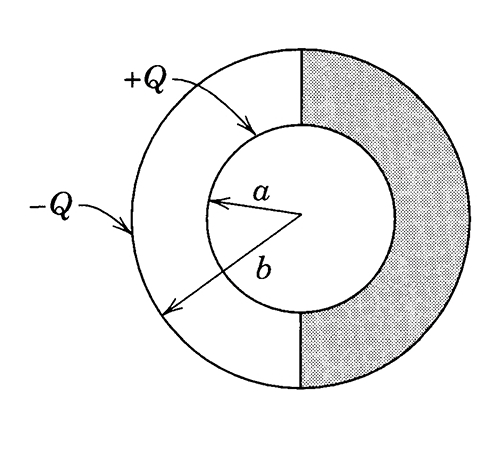
\includegraphics[width=0.3\textwidth]{hw7_p3.jpg} 
\end{center}

(a) Find the electric field everywhere between the sphere.

(b) Calculate the surface charge distribution on the inner sphere.

(c) Calculate the polarization charge density induced on the surface of the
dielectric at $r=a$.
\begin{solution}
(a) Let the system be positioned in a spherical coordinate system where the 
dielectric is located from $\theta=0$ to $\theta=\pi /2$. Then it has azimuthal
symmetry and the general solution for the potential with
$0\leq x=\cos\theta\leq 1$ is
\begin{equation}\label{p3a:Phi1}
    \Phi_{x\geq 0}=\sum_{l=0}^\infty \qty(A_lr^l+B_lr^{-(l+1)})P_l(x) 
\end{equation}
The potential is constant across the conductors. So we can evaluate
\eqref{p3a:Phi1} at $r=a$
\begin{equation}
    A_0+B_0a^{-1}+\sum_{l=1}^\infty\qty[A_la^l+B_la^{-(l+1)}]P_l(x)=V_a 
\end{equation}
where $V_a$ is some constant potential that the sphere at $r=a$ is held at.
By orthogonality, the coefficients for $l\geq 1$ must vanish and we have
\begin{equation}
    B_l=A_la^{2l+1} 
\end{equation}
Now, evaluating \eqref{p3a:Phi1} at $r=b$, we can write
\begin{equation}
    A_0+B_0b^{-1}+\sum_{l=1}^\infty A_l\qty(b^l+a^{2l+1}b^{-(l+1)})P_l(x)=V_b 
\end{equation}
where $V_b$ is some constant potential at which the sphere at $r=b$ is held. By
orthogonality, the $l\geq 1$ coefficients must vanish, so $A_l=B_l=0$ for $l\geq
1$. The potential is thus
\begin{equation}
    \Phi_{x\geq 0}=A_0+B_0r^{-1}
\end{equation}
and we can write the electric field in the northen hemisphere as
\begin{equation}
    \vb{E}_{x\geq 0}=-\grad\Phi_{x\geq0}=-\frac{A}{r^2}\rhat 
\end{equation}
where $A$ is some constant. A similar argument applies for the southern
hemisphere ($x<0$) and we can write
\begin{equation}
    \vb{E}_{x<0}=-\frac{B}{r^2}\rhat 
\end{equation}
The electric field needs to be continuous at $x=0$. Thus, $A=B$. Now, we can
calculate the electric displacement
\begin{equation}
    \vb{D}=\begin{cases}
        \epsilon\vb{E} & x\geq 0\\
        \epsilon_0\vb{E} & x<0
    \end{cases}
    =\begin{cases}
        -\frac{\epsilon A}{r^2}\rhat & x\geq 0\\
        -\frac{\epsilon_0A}{r^2}\rhat & x<0
    \end{cases}
\end{equation}
Now, by Gauss Law, the charge enclosed in a spherical Gaussian surface $S$ with
$r\in(a,b)$ is
\begin{equation}
    Q=\oint_S\vb{D}\vdot\rhat da
    =2\pi\int_{-1}^1 D r^2d(\cos\theta)
    =-2\pi A\qty[\epsilon\int_0^1d(\cos\theta)+\epsilon_0\int_{-1}^0d(\cos\theta)]
    =-2\pi(\epsilon+\epsilon_0)A
\end{equation}
Thus, we can invert for $A$ and write the electric field everywhere between the 
spheres as
\begin{equation}\label{p3a:E}
    \vb{E}=\frac{Q}{2\pi(\epsilon+\epsilon_0)}\frac1{r^2}\rhat 
\end{equation}

(b) From \eqref{p3a:E}, the electric displacement is
\begin{equation}
    \vb{D}_{x\geq
    0}=\frac{Q}{2\pi}\frac{\epsilon}{\epsilon+\epsilon_0}\frac1{r^2}\rhat 
    \qquad\text{and}\qquad
    \vb{D}_{x<
    0}=\frac{Q}{2\pi}\frac{\epsilon_0}{\epsilon+\epsilon_0}\frac1{r^2}\rhat 
\end{equation}
From (4.40, Jackson), choose $\nhat_{21}=\rhat$. So $\vb{D}_1=\bm{0}$ and
$\vb{D}_2=\vb{D}$. The free surface charge density on the sphere at $r=a$ is
thus
\begin{equation}
    \rho_{x\geq
    0}=\eval{\vb{D}_{x\geq
0}\vdot\rhat}_{r=a}=\frac{Q}{2\pi}\frac{\epsilon}{\epsilon+\epsilon_0}\frac1{a^2} 
    \qquad\text{and}\qquad
    \rho_{x<
    0}=\eval{\vb{D}_{x<0}\vdot\rhat}_{r=a}=\frac{Q}{2\pi}\frac{\epsilon_0}{\epsilon+\epsilon_0}\frac1{a^2} 
\end{equation}

(c) From (4.36, Jackson) and (4.38, Jackson), the polarization is
\begin{equation}
    \vb{P}=\epsilon_0\chi_e\vb{E}=(\epsilon-\epsilon_0)\vb{E}
    =\frac{Q}{2\pi}\frac{\epsilon-\epsilon_0}{\epsilon+\epsilon_0}\frac1{r^2}\rhat
\end{equation}
Now, at $r=a$, the normal vector to the dielectric is $\nhat_{21}=-\rhat$. Then 
the bound surface charge density on the dielectric is
\begin{equation}
    \sigma_{\text{pol}}=\vb{P}_1\vdot\nhat_{21}=-\eval{\vb{P}_{x\geq
    0}\vdot\rhat}_{r=a}
    =\frac{Q}{2\pi}\frac{\epsilon_0-\epsilon}{\epsilon_0+\epsilon}\frac1{a^2}
\end{equation}
\end{solution}
\end{problem}
%%%%%%%%%%%%%%%%%%%%%%%%%%%%%%%%%%%%%%%%%%%%%%%%%%%%%%%%%%%%%%%%%%%%%%%%%%%%%%%%
\end{document}
